\documentclass[aps,prd,reprint,showpacs,groupedaddress]{revtex4-1}
\usepackage{graphicx,color,psfrag}
\usepackage{subfigure}
\usepackage{siunitx}
\DeclareSIUnit{\yr}{\ensuremath{\mathrm{yr}}}
\usepackage{hyperref}

\newcommand{\eqnref}[1]{(\ref{eq:#1})}
\newcommand{\figref}[1]{fig.~\ref{fig:#1}}
\newcommand{\Figref}[1]{Fig.~\ref{fig:#1}}
\newcommand{\secref}[1]{section~\ref{sec:#1}}

\newcommand{\sub}[1]{\ensuremath{_\text{#1}}}
\newcommand{\super}[1]{\ensuremath{^\text{#1}}}
\newcommand{\dd}{\ensuremath{\mathrm{d}}}
\newcommand{\diff}[2]{\ensuremath{\frac{\dd {#1}}{\dd {#2}}}}
\newcommand{\intd}[4]{\ensuremath{\int_{#1}^{#2}{#3}\,\dd{#4}}}
\newcommand{\recip}[1]{\ensuremath{\frac{1}{#1}}}

\begin{document}

%\preprint{}

%Title of paper
\title{The Parabolic Limit for Peters and Matthews Energy Spectra}

\author{Christopher P. L. Berry}
\email[]{cplb2@ast.cam.ac.uk}
\author{Jonathan R. Gair}
\email[]{jgair@ast.cam.ac.uk}
\affiliation{Institute of Astronomy, Madingley Road, Cambridge, CB3 0HA, United Kingdom}

\date{\today}

\begin{abstract}
We derive an analytic expression for the gravitational wave energy spectrum for parabolic orbits using the approach of Peters and Matthews. This result is applicable in the weak-field regime, but is reasonably accurate ($\sim \SI{10}{\percent}$) provided that the orbiting body does not rotate more than $\Delta \phi = 2.2\pi$. For equatorial orbits in Kerr spacetime, this corresponds to periapse radii of $r\sub{p} \gtrsim 20 M$. The parabolic limit should be able to describe high eccentricity orbits. In particular, the results may be used for compact object scattered onto eccentric orbits about the Galactic massive black hole. The radiation from such encounters should be detectable with LISA.
\end{abstract}

% 04.30.-w 	Gravitational waves
% 04.25.Nx 	Post-Newtonian approximation; perturbation theory; related approximations
% 97.60.Lf 	Black holes
% 98.35.Jk 	Galactic center, bar, circumnuclear matter, and bulge (including black hole and distance measurements)
\pacs{04.30.-w, 04.25.Nx, 97.60.Lf, 98.35.Jk}

\maketitle

\section{Introduction}

Gravitational radiation provides an exciting, unexplored window to the Universe. Computing gravitational waveforms is a difficult task, however it is possible to derive analytic expression subject to certain simplifying assumptions. The classic work is that of Peters and Matthews\cite{Peters1963, Peters1964} (PM) who consider two point masses on Keplerian orbits.

In \secref{limit} we derive the limit of the Peters and Matthews energy spectrum for parabolic orbits.\footnote{We use ``parabolic'' to refer to marginally bound orbits. Marginally bound Keplerian orbits are parabola; in curved spacetimes they do not retain such a simple shape.} It is hoped that this analytic result can be used as a quick-and-easy method of investigating the energy flux from high eccentricity orbits, and as a means of checking that numerical codes give sensible results. The range of applicability of this result for equatorial orbits is discussed in \secref{application}.

Parabolic orbits are of astrophysical interest as they are almost indistinguishable from other high eccentricity orbits. The inspiral of compact objects (COs) towards massive black holes (MBHs), particularly the MBH in the Galactic centre, is expected to be an important source the planned NASA/ESA Laser Interferometer Space Antenna (LISA)\cite{Bender1998,Danzmann2003}. These inspirals may begin with the COs being scattered onto highly eccentric orbits by interactions with other bodies. Therefore, the parabolic limit should be a good description of the bursts of gravitational radiation emitted during the early part of the inspiral. The event rate for the detection of such bursts from the Galactic MBH with LISA has been estimated to be as high as $\SI{15}{\yr^{-1}}$\cite{Rubbo2006}, although this has been revised downwards to the order of $\SI{1}{\yr^{-1}}$\cite{Hopman2007}. Even if only a single burst is detected during the LISA mission, this is still an exciting possibility since the information carried by the GW should give an unparalleled probe of the structure of spacetime of the Galactic centre. Exactly what can be inferred will depend upon the orbit.

\section{Parabolic Limit\label{sec:limit}}

\subsection{Energy Spectrum}

For an orbit of eccentricity $e$ with periapse radius $r\sub{p}$, Peters and Matthews\cite{Peters1963} give the power radiated into the $n$th harmonic of the orbital angular frequency as
\begin{equation}
P(n) = \frac{32}{5}\frac{G^4}{c^5}\frac{M_1^2M_2^2(M_1 + M_2)(1-e)^5}{r\sub{p}^5}g(n,e)
\label{eq:PM_P}
\end{equation}
where the function $g(n,e)$ is defined in terms of Bessel functions of the first kind
\begin{eqnarray}
g(n,e) & = & \frac{n^4}{32}\left\{\left[J_{n-2}(ne) - 2eJ_{n-1}(ne) \phantom{\frac{2}{n}J_n(ne)} \right. \right. \nonumber \\*
 & & \left. + \frac{2}{n}J_n(ne) + 2eJ_{n+1}(ne) - J_{n+2}(ne)\right]^2 \nonumber \\*
 & & + \left(1 - e^2\right)\left[J_{n-2}(ne) - 2J_n(ne) + J_{n+2}(ne)\right]^2 \nonumber \\*
 & & \left. + \frac{4}{3n^2}\left[J_n(ne)\right]^2\right\}.
% Line breaks follow Peters and Matthews paper
\end{eqnarray}
The Keplerian orbital frequency is
\begin{eqnarray}
{\omega_0}^2 & = & \frac{G(M_1 + M_2)(1-e)^3}{r\sub{p}^3}\\*
 & = & (1-e)^3{\omega\sub{c}}^2,
\label{eq:Kepler_freq}
\end{eqnarray}
where $\omega\sub{c}$ is defined as the angular frequency of a circular orbit of radius $r\sub{p}$. The energy radiated per orbit into the $n$th harmonic, that is at frequency $\omega_n = n\omega_0$, is
\begin{equation}
E(n) = \frac{2\pi}{\omega_0}P(n);
\label{eq:E(n)}
\end{equation}
as $e \rightarrow 1$ for a parabolic orbit, $\omega_0 \rightarrow 0$ and the orbital period becomes infinite. The energy radiated per orbit is the total energy radiated. The spacing of harmonics is $\Delta\omega = \omega_0$, giving energy spectrum
\begin{equation}
\left.\diff{E}{\omega}\right|_{\omega_n}\omega_0 = E(n).
\end{equation}
Using the above relations, and changing to linear frequency $2\pi f = \omega$,
\begin{eqnarray}
\left.\diff{E}{f}\right|_{f_n} & = & \frac{128\pi^2}{5}\frac{G^3}{c^5}\frac{M_1^2M_2^2}{r\sub{p}^2}(1-e)^2g(n,e) \\*
 & = & \frac{4\pi^2}{5}\frac{G^3}{c^5}\frac{M_1^2M_2^2}{r\sub{p}^2}\ell(n,e),
\label{eq:PM_spectrum}
\end{eqnarray}
where the function $\ell(n,e)$ is defined in the last line. For a parabolic orbit, we must take the limit of $\ell(n,e)$ as $e \rightarrow 1$. For this we will use a number of properties of Bessel functions, and will make frequent reference to Watson\cite{Watson1995}.

We simplify $\ell(n,e)$ using the recurrence formulae (Watson\cite{Watson1995} 2.12)
\begin{eqnarray}
J_{\nu-1}(z) + J_{\nu+1}(z) & = & \frac{2\nu}{z}J_\nu(z)\\*
J_{\nu-1}(z) - J_{\nu+1}(z) & = & 2J'_\nu(z),
\end{eqnarray}
and eliminate $n$ using
\begin{eqnarray}
n & = & \frac{\omega_n}{\omega_0} \nonumber \\*
& = & (1-e)^{-3/2}\tilde{f},
\end{eqnarray}
where $\tilde{f} = \omega_n/\omega\sub{c} = f_n/f\sub{c}$ is a dimensionless frequency. Breaking $\ell$ into three manageable parts
\begin{eqnarray}
\ell & = & \underbrace{(1-e)^2n^4\left[J_{n-2} - 2eJ_{n-1} + \frac{2}{n}J_n + 2eJ_{n+1} - J_{n+2}\right]^2}_{\ell_1} \nonumber \\*
 & & + \underbrace{(1-e)^3(1+e)n^4\left[J_{n-2} - 2J_n + J_{n+2}\right]^2}_{\ell_2} \nonumber \\*
 & & + \underbrace{\frac{4(1-e)^2n^2}{3}\left[J_n\right]^2}_{\ell_3}.
\end{eqnarray}
We suppress the argument of the Bessel functions for brevity. Tackling each term of $\ell$ in turn
\begin{eqnarray}
\ell_1 & = & \left[\frac{4(1+e)\tilde{f}^2}{e}\frac{J'_n}{1-e} + 2\frac{e-2}{e}\tilde{f}\frac{J_n}{(1-e)^{1/2}}\right]^2;\\*
\ell_2 & = & 16(1+e)\left[\frac{(1+e)\tilde{f}^2}{e^2}\frac{J_n}{(1-e)^{1/2}} - \tilde{f}\frac{J'_n}{e}\right]^2;\\
\ell_3 & = & \frac{4\tilde{f}^2}{3}\left[\frac{J_n}{(1-e)^{1/2}}\right]^2.
\end{eqnarray}
To find the limit we define two new functions
\begin{equation}
A(\tilde{f}) = \lim_{e\rightarrow 1}\left\{\frac{J_n(ne)}{(1-e)^{1/2}}\right\}; \quad B(\tilde{f}) = \lim_{e\rightarrow 1}\left\{\frac{J'_n(ne)}{1-e}\right\}.
\end{equation}
To give a well defined energy spectrum, both of these must be finite. In this case we see that the second term in $\ell_2$ should go to zero.

The Bessel function has an integral representation
\begin{equation}
J_\nu(z) = \recip{\pi}\intd{0}{\pi}{\cos(\nu\vartheta - z\sin\vartheta)}{\vartheta},
\end{equation}
we want the limit of this for $\nu \rightarrow \infty$, $z \rightarrow \infty$, with $z \leq \nu$. Using the stationary phase approximation, the dominant contribution to the integral comes from when the argument of the cosine is approximately zero (Watson\cite{Watson1995} 8.2, 8.43), for small $\vartheta$
\begin{eqnarray}
J_\nu(z) & \sim & \recip{\pi}\intd{0}{\pi}{\cos\left(\nu\vartheta - z\vartheta + \frac{z}{6}\vartheta^3\right)}{\vartheta}\\*
 & \sim & \recip{\pi}\intd{0}{\infty}{\cos\left(\nu\vartheta - z\vartheta + \frac{z}{6}\vartheta^3\right)}{\vartheta};
\end{eqnarray}
this last expression is an Airy integral and has a standard form (Watson\cite{Watson1995} 6.4)
\begin{equation}
\intd{0}{\infty}{\cos(t^3 + xt)}{t} = \frac{\sqrt{x}}{3}K_{1/3}\left(\frac{2x^{3/2}}{3^{3/2}}\right),
\end{equation}
where $K_\nu(z)$ is a modified Bessel function of the second kind. Using this to evaluate our limit gives
\begin{equation}
J_\nu(z) \sim \recip{\pi}\sqrt{\frac{2(\nu - z)}{3z}}K_{1/3}\left(\frac{2^{3/2}}{3}\sqrt{\frac{(\nu -z)^3}{z}}\right).
\end{equation}
For our case
\begin{eqnarray}
\nu = (1 - e)^{-3/2}\tilde{f}; &\quad& z = (1 - e)^{-3/2}e\tilde{f}; \\*
\frac{\nu - z}{z} = (1 - e); &\quad& \frac{(\nu - z)^3}{z} = \tilde{f}^2;
\end{eqnarray}
thus
\begin{equation}
J_n(ne) \sim \recip{\pi}\sqrt{\frac{2}{3}}(1-e)^{1/2}K_{1/3}\left(\frac{2^{3/2}\tilde{f}}{3}\right),
\end{equation}
and the limiting function is well defined,
\begin{equation}
A(\tilde{f}) = \recip{\pi}\sqrt{\frac{2}{3}}K_{1/3}\left(\frac{2^{3/2}\tilde{f}}{3}\right).
\end{equation}

Finding the derivative
\begin{eqnarray}
J'_\nu(z) & = & \recip{2}\left[J_{\nu-1}(z) - J_{\nu+1}(z)\right] \nonumber \\*
 & \sim & \recip{2\pi}\left[\sqrt{\frac{2(\nu -1 - z)}{3z}}K_{1/3}\left(\frac{2^{3/2}}{3}\sqrt{\frac{(\nu - 1 - z)^3}{z}}\right) \right. \nonumber \\*
 & & \left. - \sqrt{\frac{2(\nu +1 - z)}{3z}}K_{1/3}\left(\frac{2^{3/2}}{3}\sqrt{\frac{(\nu + 1 - z)^3}{z}}\right)\right].
\end{eqnarray}
For our case
\begin{eqnarray}
\sqrt{\frac{\nu \pm 1 - z}{z}} & \simeq & (1 - e)^{1/2}\left[1 \pm \frac{(1-e)^{1/2}}{2\tilde{f}}\right];\\*
\sqrt{\frac{(\nu \pm 1 - z)^{3/2}}{z}} & \simeq & \tilde{f}\left[1 \pm \frac{3(1-e)^{1/2}}{2\tilde{f}}\right];
\end{eqnarray}
and so
\begin{eqnarray}
J'_n(ne) & \sim & \recip{2\pi}\sqrt{\frac{2}{3}}(1-e)^{1/2}\left\{\left[1 - \frac{(1-e)^{1/2}}{2\tilde{f}}\right] \right. \nonumber \\*
 & & \times K_{1/3}\left(\frac{2^{3/2}\tilde{f}}{3}\left[1 - \frac{3(1-e)^{1/2}}{2\tilde{f}}\right]\right) \nonumber \\*
 & & \left. - \left[1 + \frac{(1-e)^{1/2}}{2\tilde{f}}\right]K_{1/3}\left(\frac{2^{3/2}\tilde{f}}{3}\left[1 - \frac{3(1-e)^{1/2}}{2\tilde{f}}\right]\right)\right\}\nonumber \\*
 & \sim & -\frac{1}{2\pi}\sqrt{\frac{2}{3}}(1-e)\left[2^{3/2}K'_{1/3}\left(\frac{2^{3/2}\tilde{f}}{3}\right) \right. \nonumber \\*
 & & \left. + \recip{\tilde{f}}K_{1/3}\left(\frac{2^{3/2}\tilde{f}}{3}\right)\right].
\end{eqnarray}
We may re-express the derivative using the recurrence formula (Watson\cite{Watson1995} 3.71)
\begin{equation}
K_{\nu-1}(z) - K_{\nu+1}(z) = -2K'_\nu(z)
\end{equation}
to give
\begin{eqnarray}
J'_n(ne) & \sim & \frac{1-e}{\sqrt{3}\pi}\left[K_{-2/3}\left(\frac{2^{3/2}\tilde{f}}{3}\right) + K_{4/3}\left(\frac{2^{3/2}\tilde{f}}{3}\right) \right. \nonumber \\*
 & & \left. - \recip{\sqrt{2}\tilde{f}}K_{1/3}\left(\frac{2^{3/2}\tilde{f}}{3}\right)\right].
\end{eqnarray}
And so finally,
\begin{eqnarray}
B(\tilde{f}) & = & \recip{\sqrt{3}\pi}\left[K_{-2/3}\left(\frac{2^{3/2}\tilde{f}}{3}\right) + K_{4/3}\left(\frac{2^{3/2}\tilde{f}}{3}\right) \right. \nonumber \\*
 & & \left. - \recip{\sqrt{2}\tilde{f}}K_{1/3}\left(\frac{2^{3/2}\tilde{f}}{3}\right)\right],
\end{eqnarray}
which is also well defined.

Having obtained expressions for $A(\tilde{f})$ and $B(\tilde{f})$ in terms of standard functions, we can now calculate the energy spectrum for a parabolic orbit. From \eqnref{PM_spectrum}
\begin{equation}
\diff{E}{f} = \frac{4\pi^2}{5}\frac{G^3}{c^5}\frac{M_\bullet^2\mu^2}{r\sub{p}^2}\ell\left(\frac{f}{f\sub{c}}\right),
\label{eq:PM_dEdf}
\end{equation}
where we have used the limit
\begin{eqnarray}
\ell(\tilde{f}) & = & \left[8\tilde{f}B(\tilde{f}) - 2\tilde{f}A(\tilde{f})\right]^2 \nonumber \\*
 & & + \left(128\tilde{f}^4 + \frac{4\tilde{f}^2}{3}\right)\left[A(\tilde{f})\right]^2.
\end{eqnarray}

\subsection{Total Energy}

To check the validity of this limit we can calculate the total energy radiated. We can calculate this by integrating \eqnref{PM_dEdf} over all frequencies, or by summing the energy radiated into each harmonic. For consistency, the two approaches must yield the same result. Summing over harmonics
\begin{equation}
E\sub{sum} = \frac{64\pi}{5}\frac{G^3}{c^5}\frac{M_1^2M_2^2}{r\sub{p}^2}\omega\sub{c}(1-e)^{7/2}\sum_n g(n,e),
\end{equation}
where we have used equations \eqnref{PM_P}, \eqnref{Kepler_freq} and \eqnref{E(n)}. Peters and Matthews\cite{Peters1963} provide the result
\begin{equation}
\sum_n g(n,e) = \left(1 + \frac{73}{24}e^2 + \frac{37}{96}e^4\right)(1-e^2)^{-7/2}.
\end{equation}
Using this,
\begin{equation}
E\sub{sum} = \frac{64\pi}{5}\frac{G^3}{c^5}\frac{M_1^2M_2^2}{r\sub{p}^2}\omega\sub{c}\left(1 + \frac{73}{24}e^2 + \frac{37}{96}e^4\right),
\end{equation}
which is perfectly well behaved as $e \rightarrow 1$,
\begin{equation}
E\sub{sum} = \frac{85\pi}{2^{5/2}3}\frac{G^3}{c^5}\frac{M_1^2M_2^2}{r\sub{p}^2}\omega\sub{c}.
\label{eq:PM_total}
\end{equation}
Integrating the energy spectrum, \eqnref{PM_dEdf}, gives
\begin{equation}
E\sub{int} = \frac{2\pi}{5}\frac{G^3}{c^5}\frac{M_1^2M_2^2}{r\sub{p}^2}\omega\sub{c}\intd{0}{\infty}{\ell(\tilde{f})}{\tilde{f}}.
\end{equation}
The integral can be evaluated numerically as
\begin{eqnarray}
\intd{0}{\infty}{\ell(\tilde{f})}{\tilde{f}} & = & 12.5216858\ldots \nonumber \\*
 & = & \frac{425}{2^{7/2}3}.
\end{eqnarray}
The two total energies are consistent, $E\sub{int} = E\sub{sum}$.

\section{Applicability\label{sec:application}}

\subsection{Limit Of Approximation}

The approach of Peters and Matthews assumes Keplerian orbits in flat spacetime. This should be a valid approximation in the weak-field regime far from a massive body. To check the limit of this approximation, we may compare the PM results with those from more accurate techniques. Energy spectra for parabolic orbits do not seem to be available in the literature yet, so we will make do with the total energy fluxes calculated by Martel\cite{Martel2004a}, who uses time-domain black hole perturbation theory for a Schwarzschild black hole of mass $M$. \Figref{E_ratio} shows the ratio of the two energies as a function of periapsis distance. As expected the PM result is more accurate for larger periapses. The agreement worsens as the periapsis decreases. At $r\sub{p} = 4 M$, corresponding to the radius of the innermost stable orbit (ISO), the energy flux calculated by Martel diverges, so the ratio tends to zero. This divergence is because in Schwarzschild (or Kerr) spacetime a parabolic orbit may have a zoom-whirl structure where it undergoes a number of near circular orbits (whirls) about the black hole. As the radius of the ISO is approached, the number of whirls tends to infinity (in the absence of radiation reaction), so an infinite amount of energy is radiated.
\begin{figure*}
\subfigure[$\,$Ratio of energies verses periapse radius $r\sub{p}$.\label{fig:E_ratio}]{
\begin{psfrags}%
\psfragscanon%
%
% text strings:
\psfrag{s03}[t][t]{\color[rgb]{0,0,0}\setlength{\tabcolsep}{0pt}\begin{tabular}{c}{\Large$r_\text{p}/M$}\end{tabular}}%
\psfrag{s04}[b][b]{\color[rgb]{0,0,0}\setlength{\tabcolsep}{0pt}\begin{tabular}{c}{\Large$E_\text{PM}/E_\text{Martel}$}\end{tabular}}%
%
% xticklabels:
\psfrag{x01}[t][t]{0}%
\psfrag{x02}[t][t]{5}%
\psfrag{x03}[t][t]{10}%
\psfrag{x04}[t][t]{15}%
\psfrag{x05}[t][t]{20}%
\psfrag{x06}[t][t]{25}%
%
% yticklabels:
\psfrag{v01}[r][r]{0.0}%
\psfrag{v02}[r][r]{0.1}%
\psfrag{v03}[r][r]{0.2}%
\psfrag{v04}[r][r]{0.3}%
\psfrag{v05}[r][r]{0.4}%
\psfrag{v06}[r][r]{0.5}%
\psfrag{v07}[r][r]{0.6}%
\psfrag{v08}[r][r]{0.7}%
\psfrag{v09}[r][r]{0.8}%
\psfrag{v10}[r][r]{0.9}%
\psfrag{v11}[r][r]{1.0}%
%
% Figure:
\resizebox{7.5cm}{!}{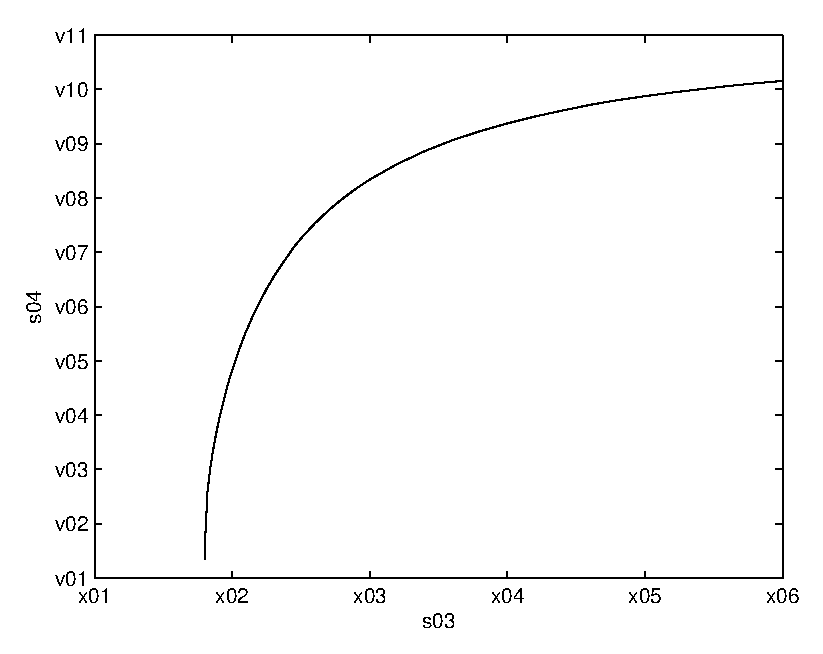
\includegraphics{E_ratio.eps}}%
\end{psfrags}%
}\qquad \qquad
\subfigure[$\,$Ratio of energies verses the reciprocal of the number of rotations $1/N$. The Keplerian limit corresponds to $N = 1$.\label{fig:N_ratio}]{
\begin{psfrags}%
\psfragscanon%
%
% text strings:
\psfrag{s03}[t][t]{\color[rgb]{0,0,0}\setlength{\tabcolsep}{0pt}\begin{tabular}{c}{\Large$1/N$}\end{tabular}}%
\psfrag{s04}[b][b]{\color[rgb]{0,0,0}\setlength{\tabcolsep}{0pt}\begin{tabular}{c}{\Large$E_\text{PM}/E_\text{Martel}$}\end{tabular}}%
%
% xticklabels:
\psfrag{x01}[t][t]{0.0}%
\psfrag{x02}[t][t]{0.2}%
\psfrag{x03}[t][t]{0.4}%
\psfrag{x04}[t][t]{0.6}%
\psfrag{x05}[t][t]{0.8}%
\psfrag{x06}[t][t]{1.0}%
%
% yticklabels:
\psfrag{v01}[r][r]{0.0}%
\psfrag{v02}[r][r]{0.1}%
\psfrag{v03}[r][r]{0.2}%
\psfrag{v04}[r][r]{0.3}%
\psfrag{v05}[r][r]{0.4}%
\psfrag{v06}[r][r]{0.5}%
\psfrag{v07}[r][r]{0.6}%
\psfrag{v08}[r][r]{0.7}%
\psfrag{v09}[r][r]{0.8}%
\psfrag{v10}[r][r]{0.9}%
\psfrag{v11}[r][r]{1.0}%
%
% Figure:
\resizebox{7.5cm}{!}{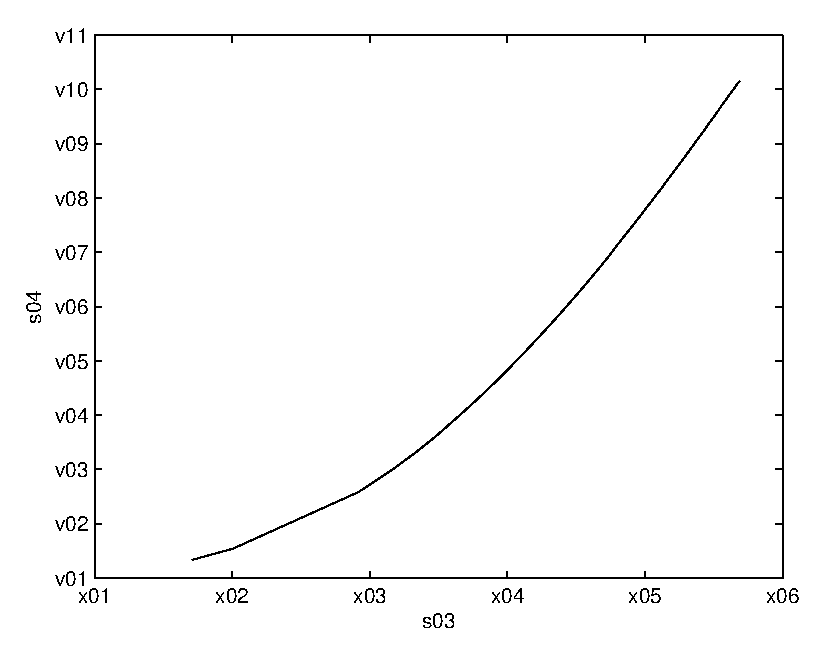
\includegraphics{N_ratio.eps}}%
\end{psfrags}%
}
\caption{Ratio of the total energy radiated as calculated using the Peters and Matthews\cite{Peters1963} approach to that calculated by Martel\cite{Martel2004a} using black hole perturbation theory. The latter approach should give more accurate results.}
\end{figure*}
\Figref{N_ratio} shows how ratio of energies correlates with the number of rotations, defined as $N = {\Delta \phi}/{2\pi}$, where $\Delta \phi$ is the total change in the azimuthal angle over an orbit. As $N$ increases the ratio decreases as the Keplerian orbit does not take into account this extra rotation. The accuracy of the PM result deteriorates rapidly once the orbit transitions to a zoom-whirl trajectory. When this happens the orbit is far from parabolic in shape.

The PM result is accurate to $\sim \SI{10}{\percent}$ for orbits with $N \lesssim 1.1$. We will adopt this as a cut-off point. For an equatorial orbit in Kerr spacetime, the number of rotations is
\begin{eqnarray}
N & = & \recip{\pi}\intd{r\sub{p}}{\infty}{\diff{\phi}{r}}{r} \nonumber \\*
 & = & \frac{L_z}{\pi\sqrt{2M}}\intd{r\sub{p}}{\infty}{\frac{r^2 - 2M(1 - a/L_z)r}{(r^2 - 2Mr + a^2)w}}{r},
\end{eqnarray}
where
\begin{equation}
w^2 = r^3 - (L_z^2/2M)r^2 + (L_z - a)^2r;
\end{equation}
$L_z$ is the angular momentum about the $z$-axis; $a$ is the spin parameter, and we have adopted units with $G = c = 1$. We will find it useful to define
\begin{equation}
r_\pm = M \pm \sqrt{M^2 - a^2},
\end{equation}
and the two non-zero roots of the cubic $w^2$
\begin{equation}
r\sub{\text{p},\,1} = \frac{L_z^2}{2M} \pm \sqrt{\frac{L_z^4}{16M^2} - (L_z -a)^2},
\end{equation}
the periapsis is the larger root $r\sub{p} > r_1$. The integral may be rewritten as
\begin{equation}
N = \frac{L_z}{\pi\sqrt{2M}}\intd{r\sub{p}}{\infty}{\recip{w}\left[1 + \frac{\alpha_+}{r-r_+} + \frac{\alpha_-}{r-r_-}\right]}{r},
\end{equation}
where
\begin{equation}
\alpha_\pm = \pm\frac{2Mar_\pm - a^2L_z}{2L_z\sqrt{M^2-a^2}}.
\end{equation}
This may be evaluated using elliptic integrals as (Gradshteyn \& Ryzhik\cite{Gradshteyn2000} 3.131.8)
\begin{eqnarray}
N & = & \frac{L_z}{\pi}\sqrt{\frac{2}{r\sub{p}M(M^2-a^2)}}\left[\left(\frac{Ma}{L_z} - \frac{a^2}{2r_+}\right)\Pi\left(\frac{r_+}{r\sub{p}}\middle|\frac{r_1}{r\sub{p}}\right) \right. \nonumber \\*
 & & \left. - \left(\frac{Ma}{L_z} - \frac{a^2}{2r_-}\right)\Pi\left(\frac{r_-}{r\sub{p}}\middle|\frac{r_1}{r\sub{p}}\right)\right],
\end{eqnarray}
where $\Pi(n|m) = \int_{0}^{\pi/2}{\dd\vartheta/(1-n\sin^2\vartheta)\sqrt{1-m\sin^2\vartheta}}$ is the complete elliptic integral of the third kind. In the limit of $a \rightarrow 0$ we recover the Schwarzschild result\cite{Cutler1994}
\begin{equation}
N = \frac{L_z}{\pi}\sqrt{\frac{2}{r\sub{p}M}}K\left(\frac{r_1}{r\sub{p}}\right),
\end{equation}
where $K(m) = \int_{0}^{\pi/2}{\dd\vartheta/\sqrt{1-m\sin^2\vartheta}}$ is the complete elliptic integral of the first kind. \Figref{N_peri} shows the periapsis for which $N = 1.1$ for a range of spins.
\begin{figure}
\begin{psfrags}%
\psfragscanon%
%
% text strings:
\psfrag{s03}[t][t]{\color[rgb]{0,0,0}\setlength{\tabcolsep}{0pt}\begin{tabular}{c}{\Large$a/M$}\end{tabular}}%
\psfrag{s04}[b][b]{\color[rgb]{0,0,0}\setlength{\tabcolsep}{0pt}\begin{tabular}{c}{\Large$r_\text{p}/M$}\end{tabular}}%
%
% xticklabels:
\psfrag{x01}[t][t]{-1.0}%
\psfrag{x02}[t][t]{-0.5}%
\psfrag{x03}[t][t]{0.0}%
\psfrag{x04}[t][t]{0.5}%
\psfrag{x05}[t][t]{1.0}%
%
% yticklabels:
\psfrag{v01}[r][r]{13}%
\psfrag{v02}[r][r]{14}%
\psfrag{v03}[r][r]{15}%
\psfrag{v04}[r][r]{16}%
\psfrag{v05}[r][r]{17}%
\psfrag{v06}[r][r]{18}%
\psfrag{v07}[r][r]{19}%
\psfrag{v08}[r][r]{20}%
\psfrag{v09}[r][r]{21}%
\psfrag{v10}[r][r]{22}%

%
% Figure:
\resizebox{7.5cm}{!}{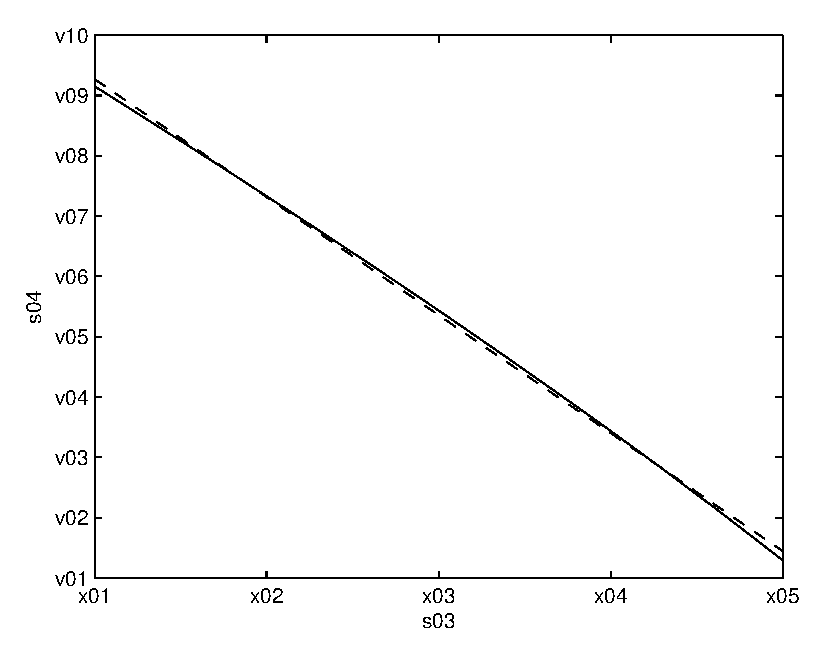
\includegraphics{N_peri.eps}}%
\end{psfrags}%
\caption{Periapsis radius corresponding to $N = 1.1$ as a function of spin parameter $a$.\label{fig:N_peri}}
\end{figure}
Equatorial orbits with larger periapses should be reasonably approximated by the PM result.

Non-equatorial orbits are more complicated because of the additional motion in the $\theta$ direction. This extra rotation will also mean that the PM approach is less accurate for non-equatorial orbits, and consequently a larger cut-off periapsis must be used.

\subsection{Astrophysical Implications}

Considering bursts from the Galactic centre, orbits with periapses of $r\sub{p} \lesssim 120 M$ should be detectable with LISA\cite{Rubbo2006, Hopman2007}. While the most interesting orbits, those which probe the strong-field region of the MBH's spacetime, are beyond the regime of the Peters and Matthews approach, $r\sub{p} \gtrsim 20 M$ for equatorial orbits, we see that many will be reasonably approximated by the PM formalism. Therefore, it should be possible to explore this region of parameter space using the PM approximation as a guide.

% If you have acknowledgments, this puts in the proper section head.
\begin{acknowledgments}
JRG's work is supported by the Royal Society. CPLB is supported by an STFC studentship.
\end{acknowledgments}

\bibliography{../library}

\end{document}
